%!TEX root = ../../main.tex

\chapter{Long tasks}
Long running tasks should generally not block the GUI. Any task that can potentially take a long time should be done on a background thread and NOT on the main GUI thread see Appendix \ref{app:threading_asynctask}. \\

Long running tasks should generally be supported by visual feedback which tells the user that something is going on and that the application is not frozen. 

\section{Progressbar}
The Android framework includes a widget called \androidinline{ProgressBar} which can be used both as an activity indicator (see Figure \ref{fig:activity_indicator_in_dialog}), and as an actual progress bar. Both usages of the word will henceforth be referred to as just \androidinline{ProgressBar}, unless otherwise made explicit. Both are great at indicating that the application is not frozen and that something is going on. The ProgressBar (as a progress bar) should generally be used when there is a reliable way of calculating the actual progress on the running task. The Activity indicator should generally be used when there is no way of telling how long there will be until the task is complete. \\

\begin{figure}[!htbp]
  \centering
    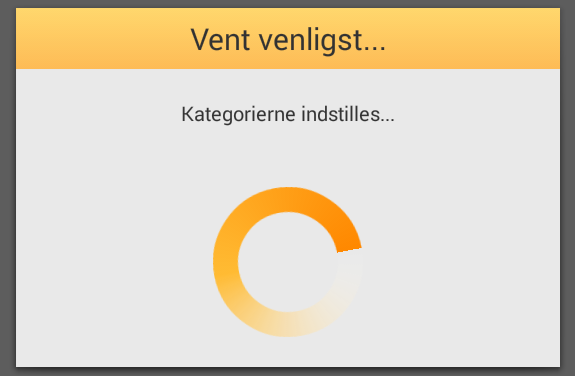
\includegraphics[width=0.8\textwidth]{progressbar_example}
    \caption{Example of a progress bar used as an activity indicator.}
    \label{fig:activity_indicator_in_dialog}
\end{figure}

\noindent If unused screen real estate is temporarily available at the location onto which elements are currently being loaded, one should place the \androidinline{ProgressBar} in this unused screen real estate.\\

\noindent If there is not enough screen real estate available, or if it does not make sense to place the \androidinline{ProgressBar} at the available location, one should use a Dialog with a \androidinline{ProgressBar} instead.